\section{Shinka Implementation Details}
\label{appsec:shinka_code}

\begin{itemize}
  \item \ouralgo uses a queue based implementation where LLMs generate program proposals sequentially. Afterwards, they are added to a job evaluation queue. Each proposal is based on all jobs that have completed so far and are stored in the database.
  \item Throughout development, we experimented with a fully asynchronous implementation that leverages both a job and a proposal queue. This allows for higher throughput but introduces a degree of "off-archiveness" in the sense that new code proposals are generated in advance and not based on all the previously submitted jobs. Furthermore, jobs from faster to query models will be executed earlier since their proposal jobs will be processed earlier. Many open research questions remain regarding the optimal trade-off between throughput, sample efficiency, and off-archiveness.
  \item Below we provide an overview of the Python API. It roughly adopts the high-level interface of \texttt{OpenEvolve} \citep{openevolve}:
\end{itemize}

\begin{minipage}{\textwidth}
\begin{lstlisting}[language=Python, basicstyle=\ttfamily\tiny, caption={Minimal \ouralgo configuration and usage example.}, label={lst:shinka_usage}]
from shinka.core import EvolutionRunner, EvolutionConfig
from shinka.database import DatabaseConfig
from shinka.launch import LocalJobConfig

# Minimal config - only specify what's required
job_config = LocalJobConfig(eval_program_path="evaluate.py")
db_config = DatabaseConfig()
evo_config = EvolutionConfig(init_program_path="initial.py",)

# Run evolution with defaults
runner = EvolutionRunner(
    evo_config=evo_config,
    job_config=job_config,
    db_config=db_config,
)
runner.run()
\end{lstlisting}
\end{minipage}

\vspace{0.5em}

\begin{minipage}{0.45\textwidth}
\textbf{\texttt{evaluate.py} - Evaluation Script}

\begin{lstlisting}[language=Python, basicstyle=\ttfamily\tiny]
from shinka.core import run_shinka_eval

def main(program_path: str,
         results_dir: str):
    metrics, correct, err = run_shinka_eval(
        program_path=program_path,
        results_dir=results_dir,
        experiment_fn_name="run_experiment",
        num_runs=3, # Multi-evals to aggreg.
        get_experiment_kwargs=get_kwargs,
        aggregate_metrics_fn=aggregate_fn,
        validate_fn=validate_fn,  # Optional
    )

def get_kwargs(run_idx: int) -> dict:
    return {"param1": "value", "param2": 42}

def aggregate_fn(results: list) -> dict:
    score = results[0]
    text = results[1]
    return {
        "combined_score": float(score),
        "public": {...},  # shinka-visible
        "private": {...},  # shinka-invisible
        "extra_data": {...},  # store as pkl
        "text_feedback": text,  # str fb
    }

if __name__ == "__main__":
    # argparse program path & dir
    main(program_path, results_dir)
\end{lstlisting}
\end{minipage}
\hfill
\begin{minipage}{0.45\textwidth}
\textbf{\texttt{initial.py} - Starting Solution}

\begin{lstlisting}[language=Python, basicstyle=\ttfamily\tiny]
# EVOLVE-BLOCK-START
def advanced_algo():
    # This will be evolved
    return solution
# EVOLVE-BLOCK-END

def run_experiment(**kwargs):
    """Main called by evaluator"""
    result = solve_problem(kwargs)
    return result

def solve_problem(params):
    solution = advanced_algo()
    return solution
\end{lstlisting}
\end{minipage}



\clearpage
\section{Task Implementation Details}
\label{appsec:implememtation}
\subsection{Circle Packing Problem}

\textbf{Detailed Task Description.} The circle packing task requires placing 26 circles within a unit square such that the sum of their radii is maximized while ensuring no circles overlap and all circles remain fully contained within the square boundary.

\begin{minipage}{0.55\textwidth}
\textbf{Verification Methodology with Slack.} For the main 
\ouralgo run presented in the paper, we employed the 
verification script provided by \texttt{OpenEvolve} \citep
{openevolve}, which allows for $1 \times 10^{-6}$ numerical 
slack. To ensure the robustness of our results, we 
additionally validated our solutions using \texttt
{AlphaEvolve}'s \citep{novikov2025alphaevolve} exact 
verification code. We found that our discovered solution can 
be made trivially exact by reducing each circle's radius by 
$1 \times 10^{-8}$, demonstrating the high precision of our 
approach. The adjustment from the relaxed to exact 
formulation reduces the sum of radii for our discovered 
solution by a negligible amount, from 2.635983099011548 to 2.
6359828390115476, representing a relative change of less than 
$10^{-6}$. 
\end{minipage}
\hfill
\begin{minipage}{0.35\textwidth}
    \centering
    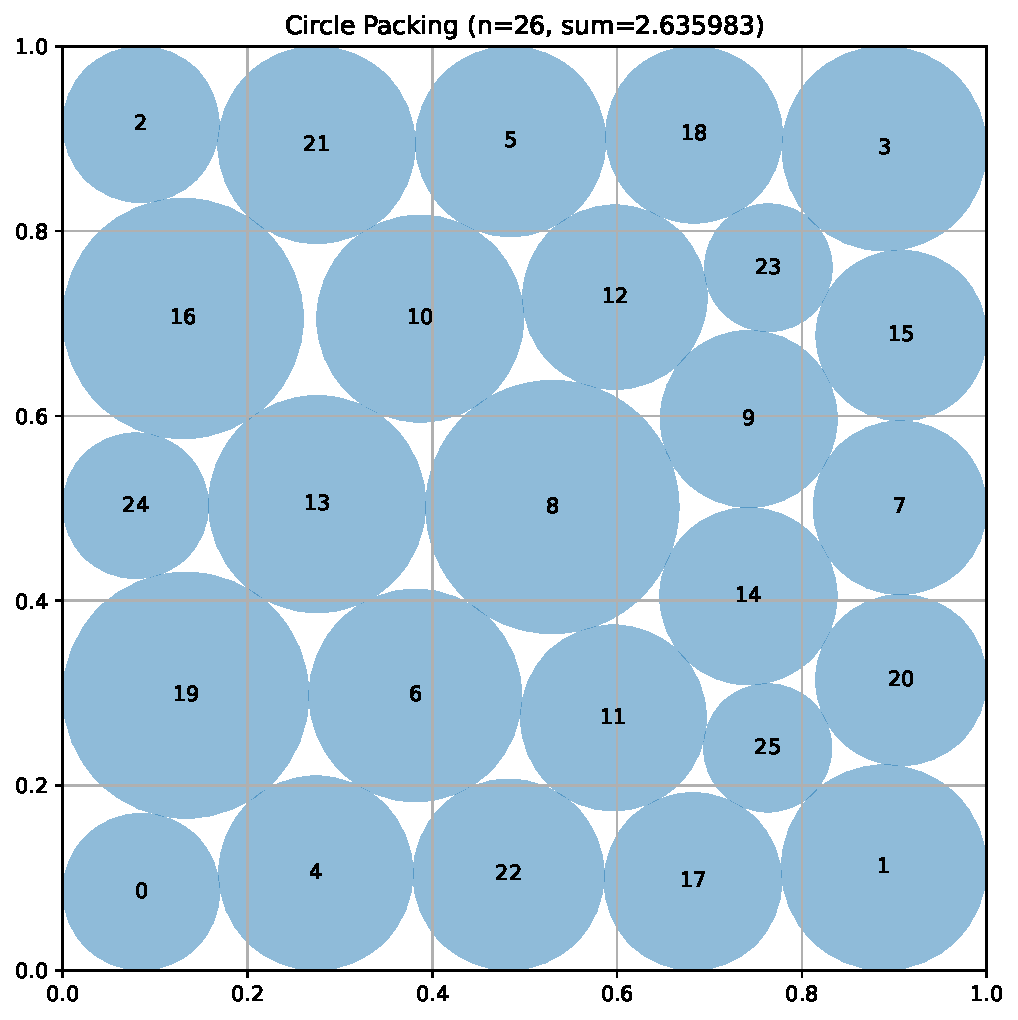
\includegraphics[height=5.5cm]{figures/circle_packing_solution.pdf}
    \captionof{figure}{Discovered Circle Packing solution by \ouralgo.}
    \label{fig:circle_packing_async_solution}
\end{minipage}

\textbf{Verification Methodology with Exact Constraint.} Additionally, we replicated the solution using the exact verification code from \texttt{AlphaEvolve} \Cref{fig:circle_packing_async} with a score of 2.63597770931127. The discovery of the solution requires more samples to be evaluated. This illustrates an important principle: surrogate relaxed tasks can be effectively used during evolution and subsequently post-processed to discover exact state-of-the-art solutions.

\begin{figure}[h]
\centering

\includegraphics[width=0.75\textwidth]{figures/circle_packing_results_async.pdf}
\caption{Circle packing asynchronous evolution results for exact circle packing verification showing convergence behavior and solution quality over time.}
\label{fig:circle_packing_async}
\end{figure}


\textbf{Baseline Comparisons.} Our performance benchmarks are established against solutions from three primary sources. The AlphaEvolve sum of radii is taken from their paper \citep{novikov2025alphaevolve}. The \texttt{OpenEvolve} baseline scores are derived from their \href{https://github.com/codelion/openevolve/tree/main/examples/circle_packing}{official implementation and examples} available in their repository. Additionally, we compare against \texttt{LLM4AD} results, specifically their \href{https://github.com/Optima-CityU/LLM4AD/blob/main/example/circle_packing/circle_packing_result.ipynb}{circle packing implementations} and \href{https://github.com/Optima-CityU/LLM4AD/blob/main/example/circle_packing/EoH_settings%26logs/run_eoh.py}{Evolution of Heuristics (EoH) experimental configurations}. These baselines provide comprehensive coverage of existing automated algorithm design approaches, enabling fair and thorough performance evaluation of our method.

\textbf{\ouralgo's Hyperparameter Configuration.}

\begin{table}[h]
\centering
\small
\begin{tabular}{lclc}
\toprule
\textbf{Parameter} & \textbf{Value} & \textbf{Parameter} & \textbf{Value} \\
\midrule
\multicolumn{4}{l}{\textbf{Database configuration}} \\
\midrule
Archive size & 40 & Elite selection ratio & 0.3 \\
Archive inspirations & 4 & Top-$k$ inspirations & 2 \\
Migration interval & 10 & Migration rate & 0.0 \\
Island elitism & true & Parent selection strategy & weighted \\
Parent selection $\lambda$ & 10.0 & Number of islands & 2 \\
\midrule
\multicolumn{4}{l}{\textbf{Evolution configuration}} \\
\midrule
Patch types & [diff, full, cross] & Patch type probs & [0.45, 0.45, 0.1] \\
Generations & 150 & Max parallel jobs & 5 \\
Max patch resamples & 3 & Max patch attempts & 3 \\
Meta recommendation interval & 10 & Max meta recommendations & 5 \\
Embedding model & text-embedding-3-small & Max novelty attempts & None \\
Code embed sim threshold & 0.95 & Problem implementation & Python \\
LLM dynamic selection & ucb1 & Exploration coefficient & 1.0 \\
\midrule
\multicolumn{4}{l}{\textbf{LLM models}} \\
\midrule
gemini-2.5-pro & $\times$ & gemini-2.5-flash & $\times$ \\
claude-sonnet-4 & $\checkmark$ & o4-mini & $\checkmark$ \\
gpt-5 & $\times$ & gpt-4.1-nano & $\checkmark$ \\
gpt-4.1 & $\checkmark$ & gpt-4.1-mini & $\checkmark$ \\
\midrule
\multicolumn{4}{l}{\textbf{LLM settings}} \\
\midrule
Temperatures & [0.0, 0.5, 1.0] & Max tokens & 16{,}384 \\
Meta models & [gpt-5-nano] & Meta temperatures & [0.0] \\
Novelty models & [gpt-5-nano] & Novelty temperatures & [0.0] \\
\bottomrule
\end{tabular}
\caption{\ouralgo{} hyperparameter configuration for the Circle Packing task.}
\label{tab:hyperparams_circle}
\end{table}

  
% EDO: changed \newpage to \clearpage to avoid other small issues rendering the appendix.
\clearpage
\subsection{AIME Math Reasoning Agentic Harness}

\begin{minipage}{0.45\textwidth}
  \paragraph{Detailed Task Description.} For the agent scaffold design task, we evaluate \ouralgo on AIME 2024 mathematical reasoning problems, consisting of 30 challenging competition-level questions requiring sophisticated problem-solving strategies \citep{AIME2024}. We limit the maximum number of LLM queries per problem to 10 for computational and cost efficiency. Using \texttt{gpt-4.1-nano} as the base model, we evolve scaffold designs over 75 generations. Additionally and to combat stochasticity in LLM queries, we evaluated each candidate evaluated across three independent runs on the complete question set. After evolution, we evaluate the discovered scaffold designs on 2023 and 2025 AIME problems \citep{AIME2023, AIME2025} to assess generalization as well as robustness to different base agent language models.
  \end{minipage}
  \hfill
  \begin{minipage}{0.45\textwidth}
      \centering
      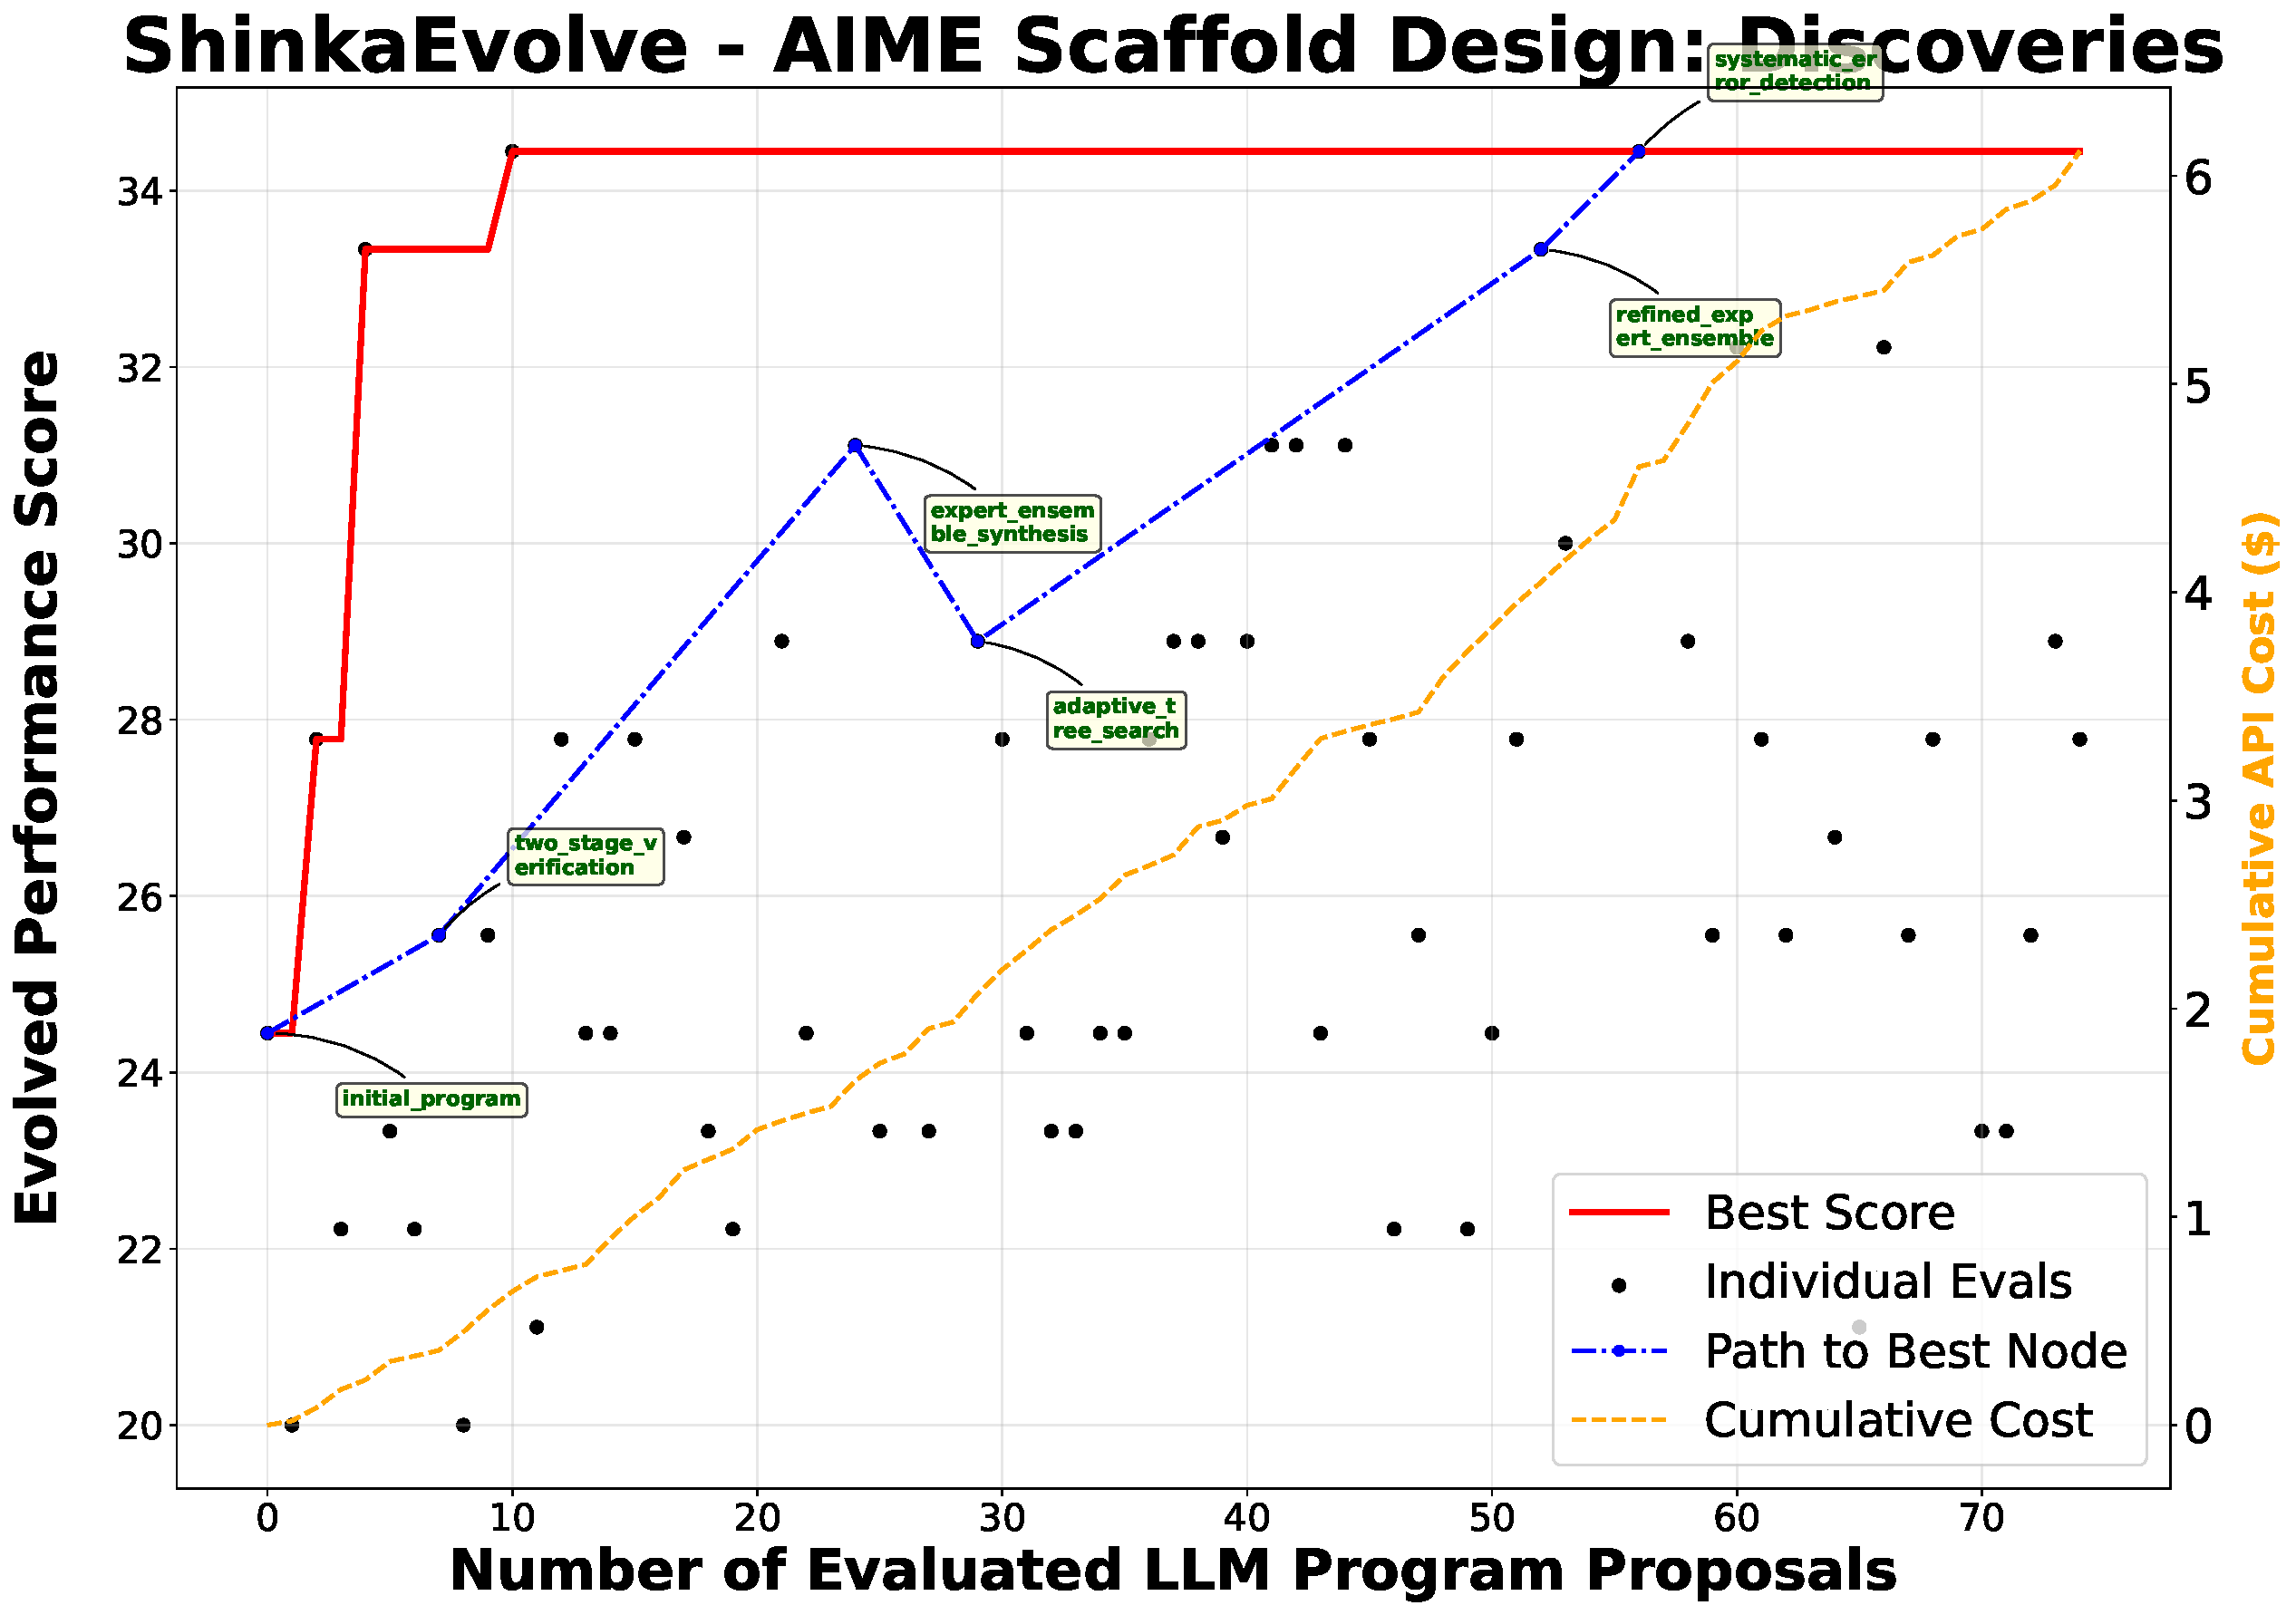
\includegraphics[height=5.5cm]{figures/aime_discoveries.pdf}
      \captionof{figure}{\ouralgo's Discovery Trajectory for Math Agent Scaffold Design.}
      \label{fig:aime_solution}
  \end{minipage}

\textbf{\ouralgo's Hyperparameter Configuration.}

\begin{table}[h]
\centering
\small
\begin{tabular}{lclc}
\toprule
\textbf{Parameter} & \textbf{Value} & \textbf{Parameter} & \textbf{Value} \\
\midrule
\multicolumn{4}{l}{\textbf{Database configuration}} \\
\midrule
Archive size & 40 & Elite selection ratio & 0.3 \\
Archive inspirations & 4 & Top-$k$ inspirations & 2 \\
Migration interval & 10 & Migration rate & 0.1 \\
Island elitism & true & Parent selection strategy & weighted \\
Parent selection $\lambda$ & 10.0 & Number of islands & 4 \\
\midrule
\multicolumn{4}{l}{\textbf{Evolution configuration}} \\
\midrule
Patch types & [diff, full, cross] & Patch type probs & [0.6, 0.3, 0.1] \\
Generations & 75 & Max parallel jobs & 1 \\
Max patch resamples & 3 & Max patch attempts & 3 \\
Meta recommendation interval & 10 & Max meta recommendations & 5 \\
Embedding model & text-embedding-3-small & Max novelty attempts & 3 \\
Code embed sim threshold & 0.95 & Problem implementation & Python \\
LLM dynamic selection & null & Exploration coefficient & 0.0 \\
\midrule
\multicolumn{4}{l}{\textbf{LLM models}} \\
\midrule
gemini-2.5-pro & $\checkmark$ & gemini-2.5-flash & $\times$ \\
claude-sonnet-4 & $\checkmark$ & o4-mini & $\checkmark$ \\
gpt-5 & $\times$ & gpt-5-nano & $\times$ \\
gpt-4.1 & $\times$ & gpt-4.1-mini & $\times$ \\
\midrule
\multicolumn{4}{l}{\textbf{LLM settings}} \\
\midrule
Temperatures & [0.0, 0.5, 1.0] & Max tokens & 16{,}384 \\
Meta models & [gpt-4.1] & Meta temperatures & [0.0] \\
Novelty models & [gpt-4.1] & Novelty temperatures & [0.0] \\
\bottomrule
\end{tabular}
  \caption{\ouralgo Hyperparameter Configuration for the Math Reasoning Agentic Harness.}
  \label{tab:hyperparams_aime}
\end{table}

\clearpage
\subsection{ALE-Bench Problems}

\paragraph{Detailed Task Description.} The ALE-Bench benchmark \citep{imajuku2025ale} is a collection of heuristic programming problems previously used in competitive programming contests (AtCoder). We evaluate \ouralgo on the LITE subset of problems, which consists of 10 problems. We follow the evaluation protocol of ALE-Agent \citep{imajuku2025ale} and use the score calculated on the public test cases as the fitness function. Afterwards, we submit the best solution to the private test set and report the score. Additionally, in \Cref{fig:results_alebench}, we provide scores for evaluating the top-5 publicly scored solutions and taking their maximum score on the private test set. While this does not resemble the traditional competitive programming setting, it allows us to assess the generalization ability of the discovered solutions. The average solution score improves by a neglible amount from 1923.5 to 1927.0. Hence, we do not observe significant evidence for overfitting to the public test cases.

\textbf{\ouralgo's Hyperparameter Configuration.}

\begin{table}[h]
\centering
\small
\begin{tabular}{lclc}
\toprule
\textbf{Parameter} & \textbf{Value} & \textbf{Parameter} & \textbf{Value} \\
\midrule
\multicolumn{4}{l}{\textbf{Database configuration}} \\
\midrule
Archive size & 50 & Elite selection ratio & 0.3 \\
Archive inspirations & 2 & Top-$k$ inspirations & 2 \\
Migration interval & 10 & Migration rate & 0.1 \\
Island elitism & true & Parent selection strategy & weighted \\
Parent selection $\lambda$ & 10.0 & Number of islands & 2 \\
\midrule
\multicolumn{4}{l}{\textbf{Evolution configuration}} \\
\midrule
Patch types & [diff, full, cross] & Patch type probs & [0.6, 0.3, 0.1] \\
Generations & 50 & Max parallel jobs & 1 \\
Max patch resamples & 3 & Max patch attempts & 3 \\
Meta recommendation interval & 5 & Max meta recommendations & 5 \\
Embedding model & None & Max novelty attempts & None \\
Code embed sim threshold & None & Problem implementation & C++ \\
LLM dynamic selection & ucb1 & Exploration coefficient & 1.0 \\
\midrule
\multicolumn{4}{l}{\textbf{LLM models}} \\
\midrule
gemini-2.5-pro & $\checkmark$ & gemini-2.5-flash & $\checkmark$ \\
claude-sonnet-4 & $\checkmark$ & o4-mini & $\checkmark$ \\
gpt-5 & $\checkmark$ & gpt-5-mini & $\checkmark$ \\
gpt-4.1 & $\times$ & gpt-4.1-mini & $\times$ \\
\midrule
\multicolumn{4}{l}{\textbf{LLM settings}} \\
\midrule
Temperatures & [0.0, 0.5, 1.0] & Max tokens & 16{,}384 \\
Meta models & [gpt-5-mini] & Meta temperatures & [0.0] \\
Novelty models & None & Novelty temperatures & None \\
\bottomrule
\end{tabular}
  \caption{\ouralgo Hyperparameter Configuration for the ALE-Bench Problems.}
  \label{tab:hyperparams_ale}
\end{table}

\clearpage
\subsection{Mixture-of-Experts Load Balancing Loss}

\paragraph{Detailed Task Description.}

\begin{table}[h]
\centering
\small
\begin{tabular}{lcc}
\toprule
\textbf{Hyperparameter} &
\textbf{Small MoE (evolution)} &
\textbf{Large MoE (evaluation)} \\
\midrule
\multicolumn{3}{l}{\textbf{Model architecture}} \\
\midrule
Model parameters & 556M & 2.7B \\
Model parameters & 82M & 404M \\
Number of experts ($N_E$) / active per token ($K$) & 64 / 8 & 64 / 8 \\
Hidden size & 512 & 1024 \\
Hidden size in each MoE expert & 384 & 768 \\
Number of hidden layers & 12 & 16 \\
Number of attention heads & 8 & 16 \\
Number of key--value heads & 8 & 8 \\
Head dimension & 128 & 128 \\
Attention bias & false & false \\
Attention dropout & 0.0 & 0.0 \\
Initializer range & 0.02 & 0.02 \\
RoPE $\theta$ & 1{,}000{,}000 & 1{,}000{,}000 \\
Tied word embeddings & true & true \\
Output router logits & true & true \\
Decoder sparse step & 1 & 1 \\
Router auxiliary loss coefficient ($\lambda$) & 0.01 & 0.001, 0.01, 0.1 \\
Computation dtype & bfloat16 & bfloat16 \\
\midrule
\multicolumn{3}{l}{\textbf{Training setup}} \\
\midrule
Optimizer & AdamW & AdamW \\
Learning rate & $1.0\times10^{-3}$ & $3.0\times10^{-4}$ \\
Weight decay & 0.1 & 0.1 \\
Adam parameters $(\beta_1,\beta_2,\epsilon)$ & (0.9, 0.95, $1\!\times\!10^{-8}$) & (0.9, 0.95, $1\!\times\!10^{-8}$) \\
Learning rate scheduler & Cosine decay & Cosine decay \\
Warmup steps & 70 & 490 \\
\midrule
Maximum sequence length & 1024 & 1024 \\
Global train batch size (sequences) & 1024 & 2048 \\
Tokens per training step & 1{,}048{,}576 & 2{,}097{,}152 \\
Maximum steps & 2000 & 14{,}000 \\
Total tokens & 2.10B & 29.36B \\
Dataset & fineweb & fineweb \\
\bottomrule
\end{tabular}
\caption{MoE architectures and training setup.}
\label{tab:moe_hparams}
\end{table}

The Mixture-of-Expert (MoE) architecture \citep{moe_sem_1, moe_sem_2, moe_mod_1_2exp, moe_mod_2_switch_1exp} has been a critical advancement, enabling scaling breakthroughs in large language model training. MoEs are currently ubiquitous amongst modern open and closed-source flagship models \citep{moe_gemini15, guo2025deepseek, llama4, moe_qwen3, moe_gemini25}. The core principle behind the MoE design is to replace traditional large feed-forward residual blocks with ensembles of smaller modules (the ``experts''), which can be efficiently sharded during training and only partially activated during inference~\citep{moe_mod_2_switch_1exp}. Each expert is itself a small feed-forward network $E_{\ell,i}$ located within a larger ensemble of size $N_E$ at layer $\ell$. The router, a layer-specific linear classifier $h_\ell$, selects the top-$K$ most relevant experts for each token, computing only their outputs:
\begin{equation}
\label{eq:moe_layer_extended}
y_\ell(x) = \sum^{N_E}_{i=1} g_{\ell,i}(x)\, E_{\ell,i}(x), \quad
g_{\ell,i}(x) =
\begin{cases}
\frac{e^{h_{\ell,i}(x)}}{\sum_{j \in \mathcal{T}_K(x)} e^{h_{\ell,j}(x)}}, & \text{if } i \in \mathcal{T}_K(x) \\
0, & \text{otherwise}
\end{cases}
\end{equation}
where $\mathcal{T}_K(x)$ denotes the set of indices corresponding to the top-$K$ router logits $h_{\ell,i}(x)$. This sparsely activated design allows different experts to specialize in distinct problem domains, enabling greater efficiency, scalability, and adaptability in handling diverse prompts.

However, due to the non-differentiability of the top-$K$ expert selection operation, it is critical to provide the router with an auxiliary load balancing loss (LBL). The LBL prevents collapse toward uneven token distributions and under-specialized experts. Devising an effective load balancing loss that simultaneously encourages efficiency and expert specialization, without hindering expressivity, remains an open design challenge that has driven much of the recent progress in MoEs~\citep{moe_sem_2, moe_mod_2_switch_1exp, moe_lbl_evo1, moe_lbl_evo2_zloss, moe_lbl_evo3, moe_deepseek_moe, moe_deepseek_demon, moe_similar_olmoe}. Minor design variations have been shown to significantly affect both efficiency and specialization ability~\citep{moe_deepseek_moe, moe_mixtral_lack_spec, moe_chameleon_lack_spec, moe_deepseek_demon_conc, moe_deepseek_demon}. 

One of the most widely adopted designs is the ``global-batch'' LBL introduced by \citet{moe_sem_2}, which underpins several state-of-the-art open models such as Qwen 3~\citep{moe_qwen3}. For a layer $\ell$ with $N_E$ experts, it is defined as:
\begin{equation}
\label{eq:moe_modern_lbl_extended}
L_{LB} = N_E \cdot \frac{1}{L}\sum_{\ell=1}^L \sum_{i=1}^{N_E} f_{\ell,i} \cdot P_{\ell,i},
\end{equation}
where
\[
f_{\ell,i} = \frac{\text{Tokens routed to expert } i}{\text{Total tokens in layer } \ell}, \qquad
P_{\ell,i} = \frac{\sum_{x} h_{\ell,i}(x)}{\sum_{x,j} h_{\ell,j}(x)}.
\]
This formulation encourages token usage across experts to align with the router’s average soft assignment probabilities.

We evaluate \ouralgo by pretraining a MoE model with 556M parameters, $N_E=64$ experts of which only $K=8$ are active for each token, corresponding to 82M sparsely activated parameters per forward pass (excluding embeddings). Training is performed on 2B tokens from fineweb~\citep{fineweb}. For each program, we define a fitness function consisting of the cross-entropy (CE) loss together with an LBL term weighted by $\lambda=0.01$. To additionally measure load imbalance, we track the L1 deviation from a uniform distribution of token allocations:
\begin{equation}
\label{eq:moe_load_imbalance_extended}
L_{\mathrm{imb}}
= \frac{1}{2}\sum_{i=1}^{N_E} \bigl|f_{\ell,i}- \tfrac{1}{N_E}\bigr| \, ,
\end{equation}
with lower values indicating more even load distribution. This grounding provides \ouralgo a two-fold search objective: minimize CE while improving load balance. To avoid local noise affecting the cross-entropy calculations, we average it over the last 10M tokens. The final fitness score used during evolution is then the negated sum of the two:
\begin{equation}
\label{eq:moe_ce_imb_tradeoff}
r= -(L_\mathrm{CE}
+ L_{\mathrm{imb}}).
\end{equation}
Given the expense of pretraining, we run \ouralgo for only 30 iterations, focusing on \texttt{gpt-4.1}, \texttt{gemini-2.5-pro}, and \texttt{claude-sonnet-4}. To evaluate generality, we scale to a larger 2.7B-parameter MoE of which 404M active (excluding embeddings), trained on slightly under 30B fineweb tokens, and compare across three LBL coefficients $\lambda \in \{0.001, 0.01, 0.1\}$. We used \texttt{AdamW}~\citep{adamw} as the optimizer with cosine decay, and linear warmup. As common practice in modern training regimes, we used rotary positional embeddings~\citep{rope}, SwiGLU MLPs~\citep{swiglu}, and half-precision bfloat16 to efficiently keep our model's weights on device. For the small model used during \ouralgo's evolution, we use a batch size of slightly over $1M$ tokens, for 2K steps. For the larger MoE used double the batch size and seven times the total number of steps. After training, we benchmark against the global-batch LBL baseline in terms of perplexity (Figure~\ref{fig:results_moe}, left) and downstream performance across seven standard evaluations: CommonSense QA \citep{moe_bench_1_commonsenseqa}, HellaSwag \citep{moe_bench_2_hellaswag}, OpenBook QA \citep{moe_bench_3_openbook_qa}, PIQA \citep{moe_bench_4_piqa}, SIQA \citep{moe_bench_5_siqa}, 
WinoGrande \citep{moe_bench_6_winogrande}, and ARC \citep{moe_bench_7_arc}, truncating the number of questions to 1000 for large benchmarks as done by~\citep{fineweb}.

\begin{wrapfigure}{r}{0.33\textwidth}
\vspace{-7mm}
\begin{center}
    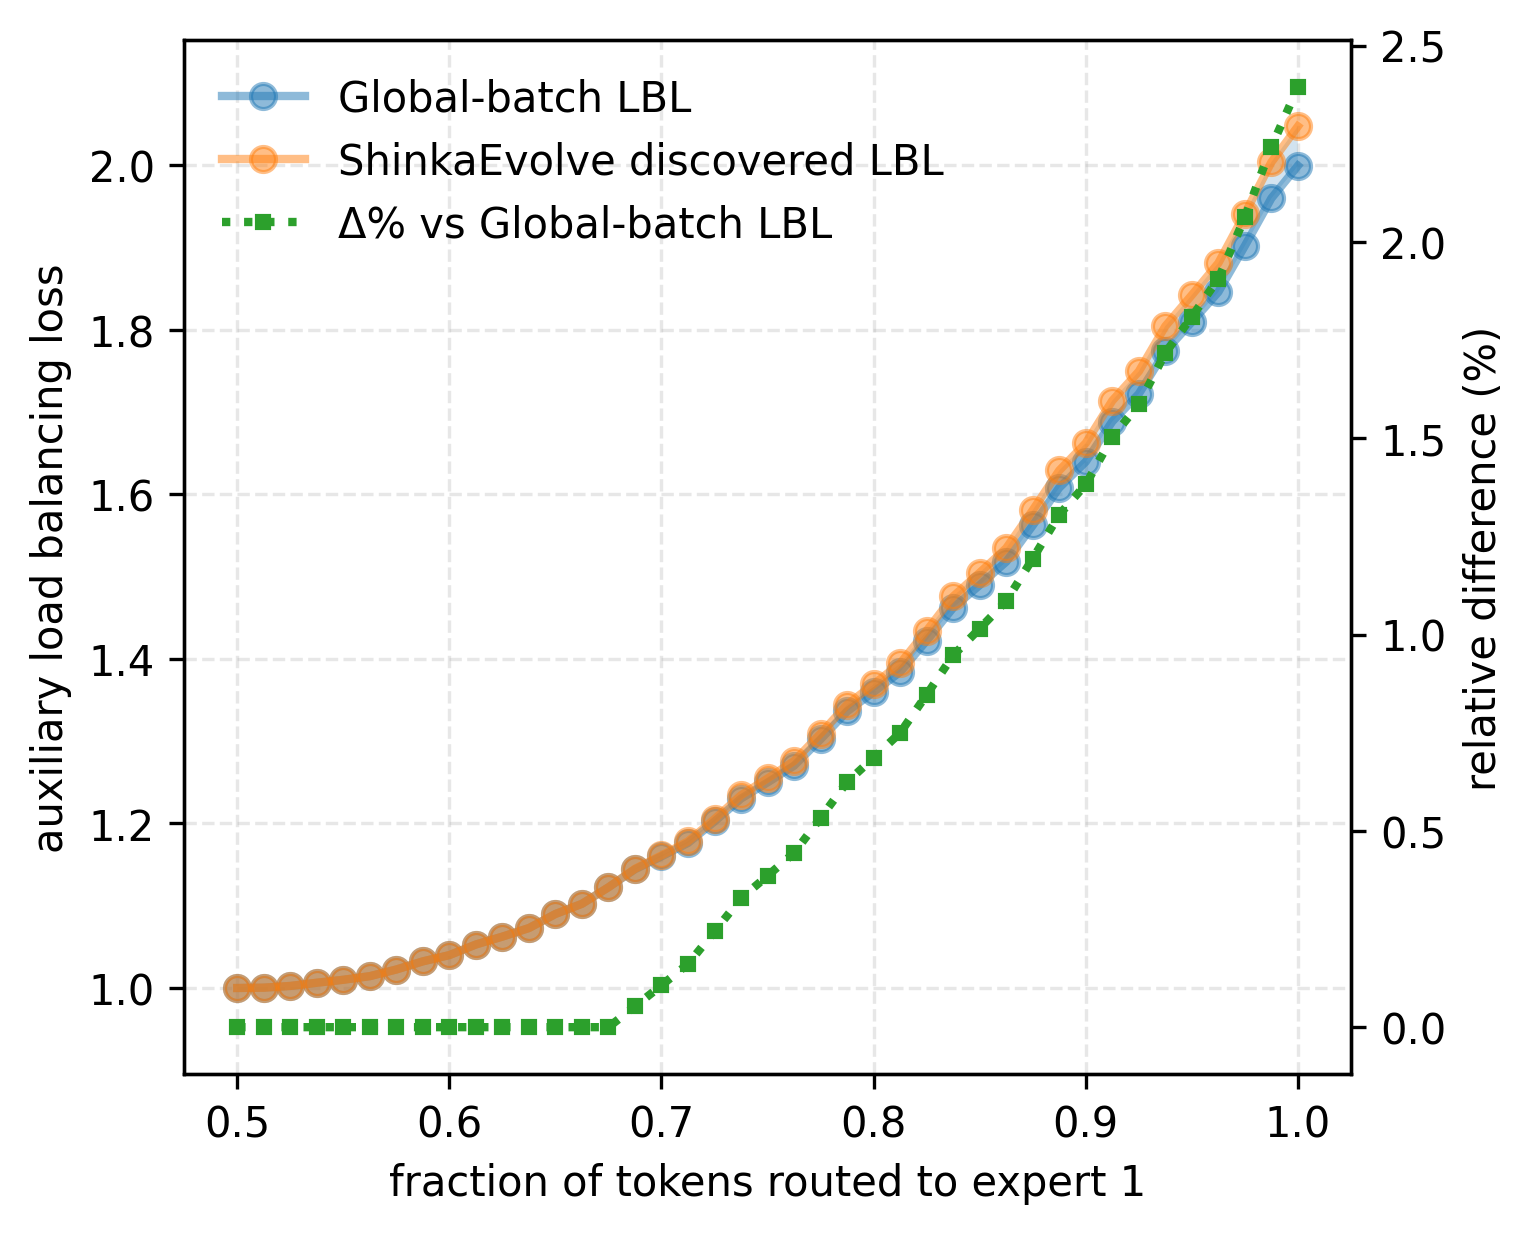
\includegraphics[width=0.33\textwidth]{figures/load_balancing_visualization_app.png}
  \end{center}
  % \vspace{-6mm}
  \caption{LBL loss comparison.}
  \label{fig:lbl_loss_value comparison}
  \vspace{-4mm}
\end{wrapfigure}


As described in Section~\ref{sec:results} and detailed in Appendix~\ref{appsec:discovered_solutions}, \ouralgo discovers a new twist on the global-batch LBL from Equation~\ref{eq:moe_modern_lbl_extended}, which was used for seeding evolutionary search. \ouralgo discovers an augmentation of this loss with an additional regularization term to target under-specialized experts. As defined in Equation~\ref{eq:moe_modern_lbl_extended}, let $f_{\ell, i}$ and $P_{\ell, i}$ denote the selection frequency and average router probabilities for expert $i$ in layer $\ell$. Furthermore, define $s(P_\ell)=0.5 + \Bigl(1-\frac{H(P_\ell)}{\log N_E}\Bigr)$ as a normalized complement of the routing entropy, and $\tau=0.064/N_E$ as a minimum usage threshold. The final discovered LBL is:
\begin{equation}
\label{eq:discovered_lbl_extended}
\begin{aligned}
L_{\mathrm{LBL}}
&=
\underbrace{%
\color{lblA} N_E \cdot \frac{1}{L}
\sum_{\ell=1}^{L}\sum_{i=1}^{N_E} f_{\ell,i}\,P_{\ell,i}
}_{\text{Global-batch LBL}}+
\underbrace{%
\color{lblB} \frac{0.1}{L}\sum_{\ell=1}^{L}
s(P_\ell)\,\sum_{i=1}^{N_E}\max\!\bigl(0,\tau-f_{\ell,i}\bigr)
}_{\text{\ouralgo new regularization}} \, .
\end{aligned}
\end{equation}

\begin{figure}[h!]
    \centering
    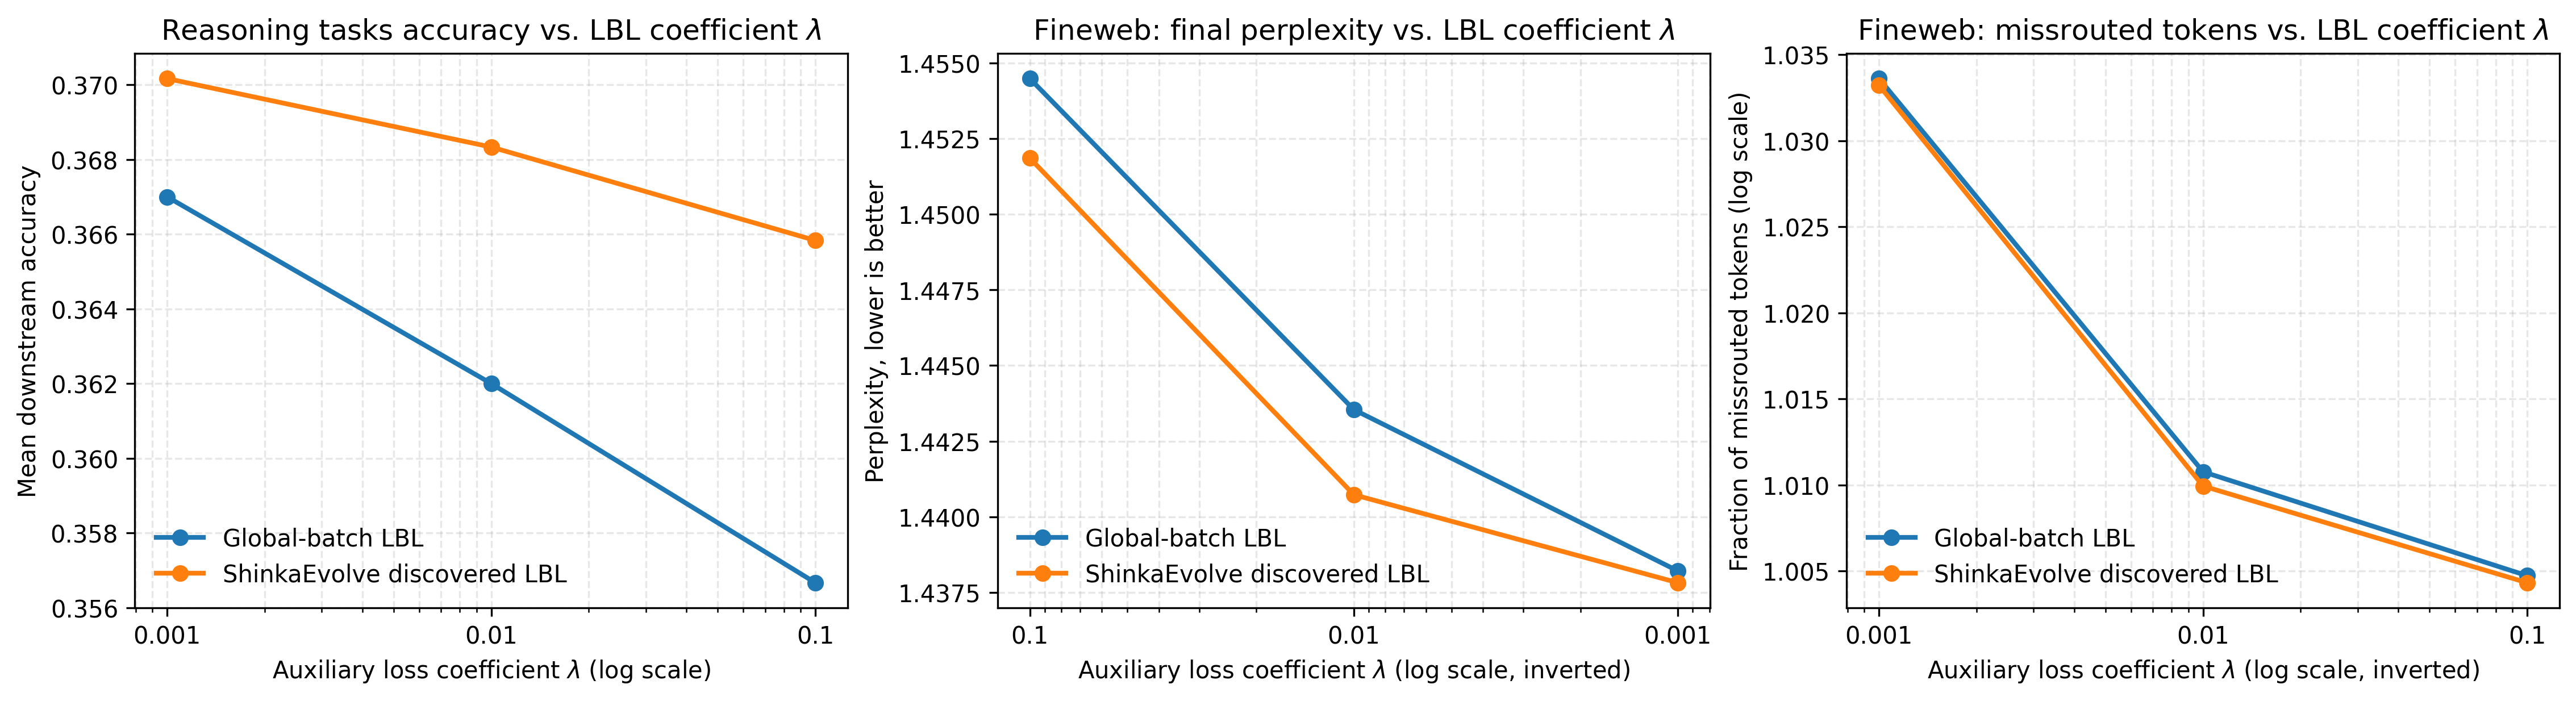
\includegraphics[width=0.975\textwidth]{figures/load_balancing_comparison_app.png}
    \caption{Mixture-of-Experts LBL design additional results.}
    \label{fig:results_moe_app}
    % \vspace{-15pt}
\end{figure}
In addition to the results from Section~\ref{sec:results}, in Figure \ref{fig:results_moe_app}, we provide additional results comparing the global-batch LBL and \ouralgo's discovered LBL. In particular, we report the average task performance, final perplexity, and the fraction of missrouted tokens, as a function of the LBL coefficient $\lambda$ used for training the MoEs. Consistent with our previous analysis, \ouralgo's LBL appears to improve from the original LBL across both axes. However, we also note that the architecture used for evolving and testing the employed LBL was quite similar, and the training budget was still limited. However, the consistent generalization results across training budgets and coefficients $\lambda$ provide an optimistic outlook for future extensions to much longer training regimes, where even small efficiency gains could scale to significant cost savings.

\clearpage
\textbf{\ouralgo's Hyperparameter Configuration.}
\begin{table}[h]
\centering
\small
\begin{tabular}{lclc}
\toprule
\textbf{Parameter} & \textbf{Value} & \textbf{Parameter} & \textbf{Value} \\
\midrule
\multicolumn{4}{l}{\textbf{Database configuration}} \\
\midrule
Archive size & 20 & Elite selection ratio & 0.3 \\
Archive inspirations & 4 & Top-$k$ inspirations & 2 \\
Migration interval & 10 & Migration rate & 0.1 \\
Island elitism & true & Parent selection strategy & weighted \\
Parent selection $\lambda$ & 10.0 & Number of islands & 2 \\
\midrule
\multicolumn{4}{l}{\textbf{Evolution configuration}} \\
\midrule
Patch types & [diff, full] & Patch type probs & [0.5, 0.5] \\
Generations & 20 & Max parallel jobs & 1 \\
Max patch resamples & 10 & Max patch attempts & 10 \\
Meta recommendation interval & 10 & Max meta recommendations & 5 \\
Embedding model & text-embedding-3-small & Max novelty attempts & 3 \\
Code embed sim threshold & 0.95 & Problem implementation & Python \\
LLM dynamic selection & ucb1 & Exploration coefficient & 1.0 \\
\midrule
\multicolumn{4}{l}{\textbf{LLM models}} \\
\midrule
gemini-2.5-pro & $\checkmark$ & gemini-2.5-flash & $\times$ \\
claude-sonnet-4 & $\checkmark$ & o4-mini & $\times$ \\
gpt-5 & $\times$ & gpt-5-nano & $\times$ \\
gpt-4.1 & $\checkmark$ & gpt-4.1-mini & $\times$ \\
\midrule
\multicolumn{4}{l}{\textbf{LLM settings}} \\
\midrule
Temperatures & [0.0, 0.5, 1.0] & Max tokens & 16{,}384 \\
Meta models & [gpt-4.1] & Meta temperatures & [0.0] \\
Novelty models & [gpt-4.1] & Novelty temperatures & [0.0] \\
\bottomrule
\end{tabular}
  \caption{\ouralgo Hyperparameter Configuration for the MoE LBL Discovery.}
  \label{tab:hyperparams_moe}
\end{table}


\clearpage

\section{\ouralgo Discovered Solutions}
\label{appsec:discovered_solutions}
\subsection{Circle Packing Problem}
\label{appsec:circle_packing}

\lstinputlisting[
  language=Python,
  caption={\ouralgo Discovered Circle Packing Solution.},
  label={lst:circle_packing},
  basicstyle=\ttfamily\tiny  % Change font size here
]{code/circle_packing.py}

\clearpage
\subsection{AIME Math Reasoning Agentic Harness}

\label{appsec:aime_agent}

\lstinputlisting[
  language=Python,
  caption={\ouralgo Discovered AIME Agent Scaffold Design.},
  label={lst:aime_agent},
  basicstyle=\ttfamily\tiny  % Change font size here
]{code/aime_agent.py}

\clearpage
\subsection{ALE-Bench Problems}

\subsubsection{ALE-Bench LITE task: \texttt{ahc039}}

\lstinputlisting[
  language=C,
  caption={\ouralgo Discovered \texttt{ahc039} Solution.},
  label={lst:ale_ahc039},
  basicstyle=\ttfamily\tiny
]{code/ahc039.cpp}

\clearpage
\subsubsection{ALE-Bench LITE task: \texttt{ahc025}}

\lstinputlisting[
  language=C,
  caption={\ouralgo Discovered \texttt{ahc025} Solution.},
  label={lst:ale_ahc025},
  basicstyle=\ttfamily\tiny
]{code/ahc025.cpp}

\clearpage
\subsection{Mixture-of-Experts Load Balancing Loss}

\lstinputlisting[
  language=Python,
  caption={\ouralgo Discovered Mixture of Experts Load Balancing Loss.},
  label={lst:aime_agent},
  basicstyle=\ttfamily\tiny
]{code/load_balancing_loss.py}